\documentclass{article}
\usepackage[utf8]{inputenc}
\usepackage{polski}
\usepackage[polish]{babel}
\usepackage{bbm}
\usepackage{amsmath}
\usepackage{amsfonts}
\usepackage{amsthm}
\usepackage{graphicx}
\usepackage{epstopdf}
\usepackage{float}
\usepackage{hyperref}
\hypersetup{colorlinks=true, urlcolor=blue}

\newtheorem{defi}{Definicja}
\newtheorem{twr}{Twierdzenie}
\newtheorem*{dd}{Dowód}

\DeclareMathOperator{\sign}{sign}
\DeclareMathOperator{\argmax}{argmax}

\newcommand{\twopartdef}[4]
{
	\left\{
		\begin{array}{ll}
			#1 & \mbox{jeśli } #2 \\
			#3 & \mbox{jeśli } #4
		\end{array}
	\right.
}


\author{Jarosław Dzikowski, Bartłomiej Najdecki}
\date{Wrocław, \today}
\title{\textbf{Projekt ze sztucznej inteligencji w grach} \\  Sztuczna inteligencja do TORCS}
\begin{document}
\maketitle

\tableofcontents

\section{TORCS}

\subsection{Czym jest TORCS}
TORCS (The Open Racing Car Simulator) to wieloplatformowy i dostępny na licencji open source trójwymiarowy symulator wyścigów samochodowych. Jest on rozwijany od 20 lat - posiada mnóstwo samochodów, torów wyścigowych. Symulacje mogą uwzględniać proste kolizje, zużycie paliwa, aerodynamikę, poślizgi i wiele więcej. Ze względu na dojrzałość API istnieje wiele rozszerzeń i dodatków. Dodatkowo co roku organizowane są zawody w programowaniu botów do symulatora.

\begin{figure}[H]
	\centering
    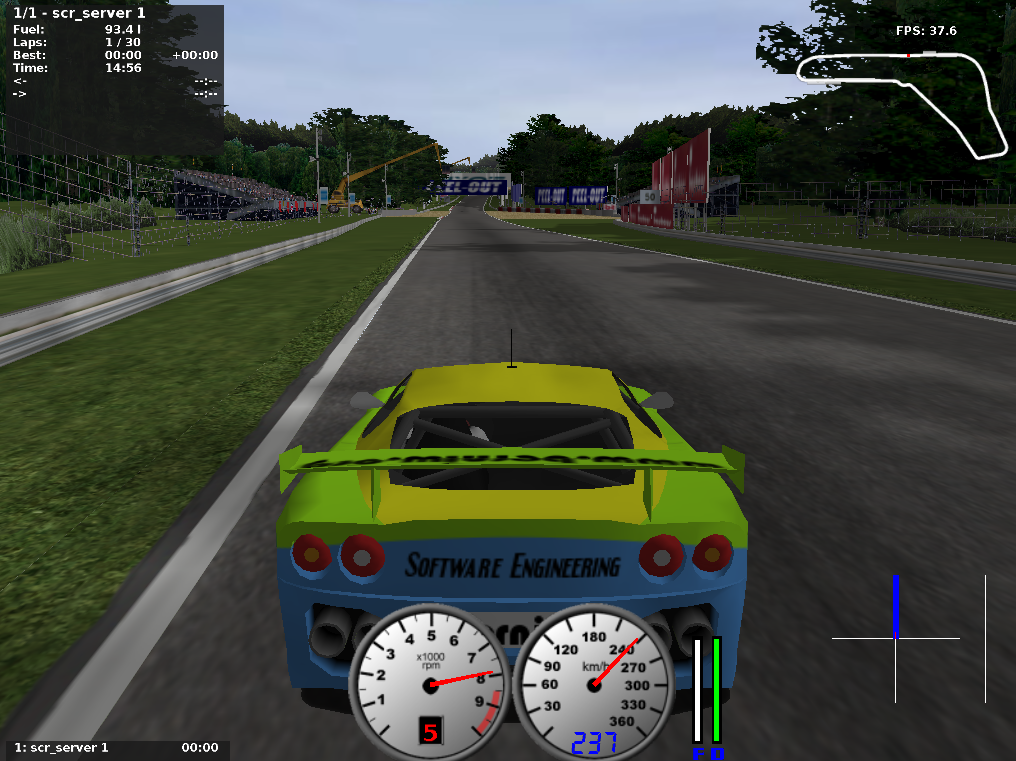
\includegraphics[width=0.8\textwidth]{torcs.png}
    \caption{Początek przejazdu okrążenia na torze Forza}
\end{figure}
\subsection{Zasady}
Gra odbywa się w czasie rzeczywistym - jeden tick gry trwa 20ms. Silnik odpytuje boty i czeka 10 ms na odpowiedź. Bot może być napisany w dowolnym języku, jednak wygodne API zostało napisane tylko do Javy i C++.\\
Zawody składają się z 3 części:\\
\begin{itemize}
\item Warm-up - 10 okrążeń na zpoznanie się z torem
\item Kwalifikacje - 3 okrążenia na czas
\item Wyścig - około 500km
\end{itemize}
\subsection{Wiedza o stanie gry}
Pełna tabela informacji dostępnych w trakcie gry znajduje się w bibliografii, tutaj znajduje się skrócona lista najistotniejszych elementów:
\begin{itemize}
\item distFromStart - dystans wzdłuż linii toru, który przejechaliśmy od startu
\item gear - bieg w samochodzie
\item rpm - obroty silnika
\item speedX, speedY, speedZ - odpowiednio prędkość samochodu równolegle do kierunku jazdy,  prędkość pozioma, prostdła do kierunku jazdy oraz prędkość pionowa
\item track - wektor 19 sensorów oznaczające odleglości krawędzi toru/innych samochodów. Ustawiamy kąty pod jakimi są ustawione sensory na początku wyścigu. Maksymalny zasięg widzenia sensorów to 200m. Dodatkowo w trakcie wyścigu sensory są zaburzane szumem o rozkładzie normalnym i odchyleniu 10%.
\item trackPos - pozycja na torze. -1 oznacza prawą krawędź tory, +1 lewą krawędź. Gdy \(|trackPos| > 1\), to jesteśmy poza torem.
\end{itemize}
\subsection{Możliwe Akcje}
\begin{figure}[H]
	\centering
    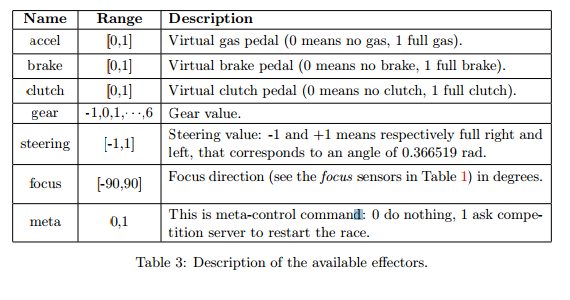
\includegraphics[width=0.8\textwidth]{inputs.png}
    \caption{Tabelka przedstawia dane, które dostajemy co tick gry.}
\end{figure}

\section{Metody sztucznej inteligencji}
\subsection{Metody heurystyczne}
Każda z metod w tej sekcji jest oparta na prostej heurystyce przy wybieraniu toru jazdy - zawsze jeźdzmy w tą stronę w którą mamy największą wolną przestrzeń(sensor pokazuje największą wartość).
\subsubsection{Podejście 1}

Ta prosta heurystyka daje dość dobre przybliżenie optymalnego toru - samochód bardzo dobrze ścina zakręty, jednak nie zawsze dobrze się do nich ustawia.
Dzięki zastosowaniu tej funkcji znacznie upraszczamy problem - wystarczy jedynie dobrze ustalać prędkości wchodzenia i wychodzenia z zakrętów. W pierwszym podejściu prędkość jest ustalana na podstawie wartości \(c_{min}\) zdefiniowanej następująco:\\
\[c_{min} = min { T(-15), T(-10), T(-5), T(0), T(5), T(10), T(15)} \]
gdzie \(T(x)\) oznacza track-sensor ustawiony pod kątem x stopni.\\
Oto tabelka przedstawiająca znalezione przeze mnie wartości, które pozwalają w miarę bezpiecznie (bez wyjeżdżania poza granice toru) zrobić okrążenie w rozsądnym czasie:

\begin{tabular}{|r|l|} \hline
\(c_{min}\) & maksymalna prędkość\\
\hline 
\(>150\)    & max \\
(100, 150] & 260 km/h \\
(60, 100] & 220 km/h \\
(50, 60] & 150 km/h \\
(40, 50] & 120 km/h \\
(30, 40] & 100 km/h \\
(20, 30] & 85 km/h \\
(0, 20] & 70 km/h \\
\hline 
\end{tabular}\\\\
Dzięki tak dobranym parametrom, samochód jest w stanie przejeżdżać okrążenie na torze Forza w czasie 2 min (boty robią to w czasie ~1 min 30 s). Z moich obserwacji wynika, że bardzo często samochód za wolno jechał przez pewne sekcje torów - niezbędne było inne podejście.
\subsubsection{Podejście 2}
Bez znajomości toru nie są możliwe drastyczne zmiany prędkości - zwiększanie prędkości granicznych powodowało wypadanie w innych sekcjach toru. Z tego powodu algorytm uległ zmianie - pierwsze okrążenie samochód przejeżdża okrążenie algorytmem starym algorytmem zapamiętując miejsca w których zaczynają się i kończą zakręty oraz prędkości z jakimi w nie wszedł. Następnie co okrążenie próbuje zwiększyć każdą z tych prędkości o zmniejszającą się wartość \(K\). Jeśli samochód po zwiększeniu prędkości wypadnie z toru nie zwiększamy wartości przypisanych sekcji toru. Oto kilka czasów z przykładowego przejazdu po torze Forza:\\

\begin{tabular}{|r|c|c|} \hline
Nr okrążenia & Czas (minuty:sekundy:milisekundy) & Ilość wypadnięć\\
\hline 
1 & 2:00:190 & 0 \\
2 & 1:59:930 & 1 \\
3 & 2:10:830 & 2 \\
4 & 2:09:370 & 2 \\
5 & 1:50:970 & 0 \\
6 & 2:06:540 & 2 \\
7 & 1:48:790 & 0 \\
12 & 1:46:710 & 0 \\
17 & 1:42:610 & 0 \\
\hline 
\end{tabular}\\\\

Czasy zostały znacznie poprawione. Samochód odczytuje obecną odległość do zakrętu i oblicza drogę potrzebną do zwolnienia do zadanej prędkości - na tej podstawie decyduje czy zwolnić czy przyspieszyć. Uzyskane czasy są zadawalające, jednak ich wyuczenie trwa długo i mocno zależy od toru.
\subsection{Uniwersalny Q-Learning}

Celem tej metody jest nauczenie komputera wydajnego jeżdżenia samochodem na dowolnej trasie.

\subsubsection{Q-Learning oraz Decyzyjne Procesy Markova}
Q-Learning jest metodą uczenia się ze wzmocnieniem służącą do wyznaczania optymalnej polityki w dowolnym skończonym Decyzyjnym Procesie Markova (Markov Decision Process). Każdy MDP składa się z pięciu części: zbioru stanów $S$, zbioru akcji $A$, które można podejmować w stanach, rozkładu prawdopodobieństwa $P_a(s, s')$ oznaczającego jaka jest szansa, że po wykonaniu akcji $a$ w stanie $s$ znajdziemy się w stanie $s'$, funkcji $R_a(s,s')$ oznaczającej nagrodę za wykonanie akcji $a$ w stanie $s$ i znalezieniu się w stanie $s'$, oraz współczynnika dyskontowania $\gamma \in [0,1]$ reprezentującego ważność przyszłych nagród. Rozwiązaniem MDP jest optymalna polityka $\pi' : S \mapsto A$ wyboru akcji maksymalizująca sumę nagród częściowych (Nagród uzyskiwanych w trakcie wędrówki po przestrzeni stanów). $\pi'(s)$ oznacza optymalną akcję, którą należy wykonać w stanie $s$.

W wielu problemach, które można reprezentować jako MDP, rozkład prawdopodobieństwa jest nieznany i często niemożliwy do obliczenia. Właściwością metody Q-Learning jest to, że nie wymaga ona znajomości rozkładu prawdopodbieństwa $P_a(s,s')$. Q-Learning polega na wyznaczeniu funkcji $Q : S \times A \mapsto \mathbb{R}$, gdzie $Q(s,a)$ reprezentuje użyteczność wykonania akcji $a$ w stanie $s$. W Q-Learningu zaczynamy z użytecznościami równymi zero, następnie rozpoczynamy wędrówkę po przestrzeni stanów ze stanu początkowego $s_{init}$ wykonując akcje według pewnej polityki $\pi$. Często wykorzystywana w Q-Learningu jest polityka $\epsilon$-greedy, w której z prawdopodobieństwiem $\epsilon$ wybierana jest losowa akcja, a z prawdopodobieństwem $1 - \epsilon$ akcja z największą użytecznością, tj. $\argmax_{a \in A} Q(s, a)$. Z każdym przejściem między stanami wiąże się tymczasowa nagroda - ponieważ dążymy do odnalezienia polityki maksymalizującej sumę nagród, musimy uwzględnić otrzymaną nagrodę w użyteczności wykonanej akcji w stanie, z którego przyszliśmy. Funkcję $Q$ aktualizuje się następująco:
\begin{equation}
Q(s,a) \leftarrow Q(s,a) + \alpha(R_a(s,s') + \gamma \max_{a' \in A} Q(s',a') - Q(s,a)) ,
\end{equation}
gdzie $\alpha$ jest współczynnikiem nauki, $s'$ jest stanem, w którym się znaleźliśmy po wykonaniu akcji $a$ w stanie $s$, a $\gamma$ jest współczynnikiem dyskontowania znanym nam z procesów Markova. Współczynnik nauki $\alpha \in (0,1)$ odpowiada za to jak wielkie znaczenie na naszą funkcję użyteczności ma jeden ,,eksperyment'' wykonania akcji $a$ w stanie $s$. Współczynnik dyskontowania $\gamma$ opisuje jak bardzo interesują nas przyszłe nagrody: im mniejszy współczynnik, tym bardziej interesują nas tymczasowe nagrody - wędrujemy po przestrzeni stanów zachłannie.

W taki oto sposób wykonujemy wiele przebiegów uczących: każdy przebieg zaczyna w stanie $s_{init}$, wędruje po przestrzeni stanów $S$, a kiedy trafiamy na stan terminalny, to uruchamiamy kolejny przebieg uczący. Im więcej przebiegów uczących zostanie wykonanych, tym lepsza będzie wyuczona funkcja użyteczności $Q$.

\subsubsection{Model Q-Learningu w TORCS}

\paragraph{Przestrzeń stanów:}
Aby móc przeprowadzić uczenie za pomocą Q-Learningu potrzebne jest umodelowanie przestrzeni stanów oraz akcji. Intuicyjnie, podjęta przez komputer akcja powinna zależeć od czynników takich jak kształt odcinka toru przed samochodem oraz prędkość z jaką porusza się samochód: gdy jedziemy po prostej, możemy wcisnąć gaz do dechy, a kiedy widzimy, że zbliża się zakręt, zwalniamy (Pod warunkiem, że jedziemy za szybko). W takim wypadku możemy reprezentować stan jako para (kształt odcinka toru, prędkość). O ile prędkość jest skalarem, to należy zastanowić się jak reprezentować kształt odcinka toru bezpośrednio przed nami. Można tutaj wykorzystać informacje, które zapewnia interfejs botów: zestaw sensorów toru. Mamy do dyspozycji 19 sensorów umieszczonych symetrycznie pod kątami z przedziału [-90 deg, 90 deg]. Każdy sensor daje nam informację jak daleko znajduje się krawędź toru pod danym kątem, lecz maksymalny zasięg sensora wynosi 200m. Mamy zatem wektor dziewiętnastu liczb rzeczywistych, które mogą posłużyć nam za reprezentacje kształtu odcinka toru. 

Pojawia się problem nieskończoności oraz wymiarowości przestrzeni stanów: $s \in \mathbb{R}^{19} \times \mathbb{R}^{1} \sim \mathbb{R}^{20}$. Przestrzeń stanów należy zamienić w przestrzeń skończoną oraz zmniejszyć wymiar stanu. Jeśli chodzi o prędkość, to łatwo ją zdyskretyzować: przestrzeń $\mathbb{R}$ możemy podzielić na przedziały, np. $\{$($-\infty$), 0), [0, 30), [30, 80), (80, $+\infty$)]$\}$, a następnie myśleć tylko o numerze przedziału prędkości, w którym się znajdujemy.

Co do redukcji wymiarowości oraz dyskretyzacji przestrzeni kształtów odcinków toru, to proponujemy nieco bardziej skomplikowane podejście. Zebrawszy uprzednio wielki zbiór danych różnych odczytów dziewiętnastu sensorów, grupujemy odczyty (wektory w $\mathbb{R}^{19}$) za pomocą algorytmu K-Means, który wyznacza centroidy grup - każdy centroid jest wektorem reprezentującym swoją grupę. Zestaw danych możemy pogrupować na dowolną liczbę grup. Aby wyznaczyć do której grupy należy aktualny stan sensorów samochodu, znajdujemy najbliższy w sensie metryki euklidesowej centroid, a następnie zapamiętujemy jego identyfikator, czyli de facto identyfikator grupy, do której przynależy aktualny stan sensorów.

\begin{figure}[H]
	\centering
    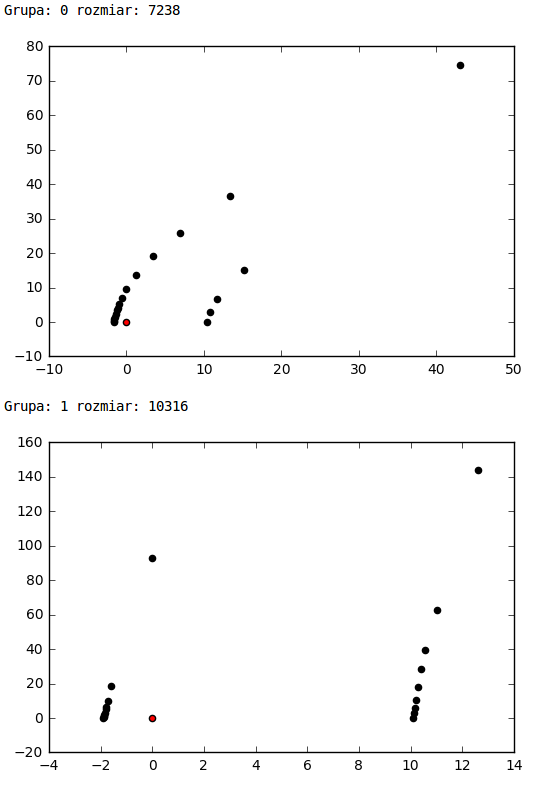
\includegraphics[width=0.8\textwidth]{exampleCentroids.png}
    \caption{Dwa przykładowe centroidy reprezentujące dwie grupy kształtów odcinków toru przy grupowaniu algorytmem K-Means (K = 120). Czarne kropki reprezentują odczyty z dziewiętnastu sensorów, czerwona kropka przedstawia pozycję samochodu, który ustawiony jest zawsze wzdłuż osi Y.}
\end{figure}

Po zastosowaniu powyższych technik przestrzeń stanów jest reprezentowana jako para liczb naturalnych ($\mathbb{N} \times \mathbb{N}$), gdzie pierwszą współrzędną jest identyfikator grupy, do której należy kształt odcinka toru przed samochodem, a drugą numer przedziału prędkości, do którego należy aktualna prędkość samochodu.

\paragraph{Przestrzeń akcji:}
Dla uproszczenia problemu, odpuścimy sobie manipulację sprzęgłem oraz będziemy używać automatycznej skrzyni biegów. Sterujemy zatem samochodem używając tylko kierownicy (Wartość skrętu z przedziału $[-1,1]$), pedałem gazu (Wartość z $[0,1]$) oraz hamulcem (Wartość z $[0,1]$). Dodatkowo założymy, że nigdy nie gazujemy oraz hamujemy jednocześnie. Jeśli chodzi o akcje skrętu, to w naszym modelu wystarczy wybrać sobie kilka konkretnych skrętów (Np. 0, -0.1, +0.1, -0.5, +0.5). Zbiór akcji gazowania/hamowania możemy ograniczyć do wartości z przedziału $[-1,1]$, gdzie -1 oznacza pełne wciśnięcie hamulca, a +1 oznacza pełne wciśnięcie gazu. W naszym modelu wyróżniamy trzy akcje gazowania/hamowania: -1, 0, 1.

\paragraph{Funkcja nagrody:}
Ostatnią rzeczą potrzebną do umodelowania środowiska do Q-Learningu jest funkcja nagrody, na podstawie której nasz bot będzie się uczył, które akcje są opłacalne, a które nie. Żeby wyprowadzić taką funkcję, należy uprzednio ustalić jakie efekty chcemy osiągnąć. 

Przede wszystkim, nie chcemy by samochód wyjechał poza tor - funkcja nagrody powinna surowo karać takie sytuacje zwracając dużą ujemną nagrodę. Stan, w którym samochód wyjeżdża poza tor jest terminalny - wracamy wtedy na linię startu i rozpoczynamy kolejny przebieg uczący. Żeby uniknąć negatywnej nagrody, uczący się bot mógłby po prostu stać miejscu i zadowolić się zerową nagrodą. Aby tego uniknąć wprowadzamy kolejną surową ujemną nagrodę w przypadku, kiedy między przejściem ze stanu $s$ do stanu $s'$ przejechany dystans nie przekroczył progu akceptowalnej przebytej drogi. Chcemy, by nasz bot jeździł wydajnie - im szybciej, tym lepiej, dlatego wprowadzamy dla zachęty dodatnią nagrodę, którą jest przebyta odległość między stanem $s$ a staniem $s'$. Im większa przebyta odległość, tym większa prędkość samochodu, tym większa nagroda.

Dobranie wartości kary za wyjechanie poza tor, wartości kary za ,,stanie w miejscu'' oraz ustalenie progu minimalnej drogi, którą należy przebyć między dwoma stanami jest zadaniem użytkownika.

\subsubsection{Jazda z wyuczoną polityką}
Kiedy już zdecydujemy, że komputer nauczył się jeździć wystarczająco dobrze, musimy wykorzystać utworzoną funkcję użyteczności $Q$ do konstrukcji polityki optymalnej $\pi'$. Z tego powodu zaimplementowany został bot, który wczytuje z pliku wyuczoną funkcję $Q$ oraz będąć w danym stanie wykonuję akcję, która ma największą użyteczność, tj. $\argmax_{a \in A} Q(s, a)$.

Niestety, jak się okazuje, polityka $\pi'$ nie zawsze chroni nas od wyjechania poza tor. W celu powrotu na trasę zostałą wykorzystana procedura powrotu zaimplementowana w prostym, naiwnym bocie domyślnie dołączanym do TORCS'a.

Ciekawym podejściem do ostatecznej polityki jazdy jest skonstruowanie rozmytej polityki jazdy $\pi_{rozm}$. W odróżnieniu od zachłannej polityki $\pi'$, polityka $\pi_{rozm}$ bierze $K$ najbliższych stanów oraz konstruuje finalną akcję jako średnią ważoną z najlepszych akcji w $K$ najbliższych stanach. Im bliższy stan, tym większą wagę ma jego akcja. Najbliższe stany można wybierać względem grup kształtów odcinków trasy, do których przynależy nasz aktualny odczyt z sensorów samochodu, lub względem przedziałów prędkości. Polityka, która bierze średnią ważoną najlepszych akcji wśrod $K$ stanów o najbliższym kształcie odcinka toru oraz uwzględnia najlepsze akcje nie tylko w przedziale prędkości, w którym znajduje się samochód, ale także w sąsiadujących przedziałach, nazywana będzie polityką $\pi_{rozm+speed}$.

\subsubsection{Testy}
Ponieważ ticki serwera gry zdarzają się 100 razy na sekundę, akcje wybierane w learningu są stosowane przez 10 kolejnych ticków, a aktualizacja funkcji użyteczności następuje podobnie tylko raz na 10 ticków. Powodem ku temu jest fakt, że stan, w którym znajduje się samochód nie zmieni się znacznie w przeciągu jednej setnej sekundy, przez co będziemy często aktualizować użyteczność jakiejś akcji w stanie $s$ korzystając z użyteczności wszystkich akcji w $s$.

\paragraph{Pierwsze podejście}

Przestrzeń stanów zawiera 120 grup kształtów odcinków toru oraz 7 przedziałów prędkości: 0-10, 10-30, 30-80, 80-110, 110-150, 150-200, 200-$\infty$. Przestrzeń akcji skrętów zawiera 5 możliwości: skręt -0.5, -0.1, 0, +0.1, +0.5, a akcje gazowania / hamulców są takie same jak opisano wcześniej. Dodatkowo współczynnik nauki $\alpha = 0.1$, współczynnik dyskontowania $\gamma = 0.99$, a szansa na podjęcie losowego ruchu w polityce $\epsilon$-greedy wynosi $\epsilon = 0.05$. Kara za opuszczenie toru wynosi -10, kara za bezruch wynosi -20, a próg bezruchu wynosi 0.1m.

Przy tej konfiguracji komputer uczył się przez około dwa tygodnie. Wybrana została trasa Wheel 2 zapewniająca wiele zakrętów różnych trudności w celu wyuczenia się odpowiedniego zachowania w różnych sytuacjach na drodzę. Początkowo uczący się komputer stoi w miejscu chaotycznie wykonując losowe akcje w celu odkrycia, które akcje dają jakieś ciekawe efekty (Pozytywną nagrodę). Kolejna faza uczenia, w którą wchodzi komputer jest przejeżdżanie bardzo wolno coraz to większej części toru wyścigowego. Już kilka godzin od rozpoczącia nauki, komputer potrafi przejechać okrążenie bez wypadania poza tor w czasie około 500 sekund, czyli bardzo wolno. Dla porównania człowiek potrafi przejechać tę samą trasę w około 140 sekund bez uprzedniego treningu. W miarę upływu czasu komputer uczył się jeździć co raz szybciej, o czym świadczyła liczba ticków serwera między początkiem każdego przebiegu uczącego a wypadnięciem samochodu poza tor. W efekcie bot przejeżdżał całe okrążenie coraz rzadziej, lecz ze zmniejszającym się czasem. Uzyskany rekord po dwóch tygodniach nauki wynosił około 215 sekund.

Testy odbyły się na dwóch torach: na torze Wheel 2, na którym bot uczył się jeździć, oraz na torze Forza (Całkiem prosty tor umożliwiający szybką jazdę). Na torze Forza bot jeżdżący z użyciem polityki optymalnej $\pi'$ uzyskał najlepszy czas 3:07, czyli 187 sekund. Bot jeżdżący z użyciem rozmytej polityki biorącej pod uwagę 3 najbliższe stany uzyskał dużo lepszy czas - 2:30, czyli 150 sekund. Bot z rozmytą polityką uwzględniającą także najlepsze akcje ze stanów z sąsiadującymi przedziałami prędkości osiągnął czas 2:33, czyli podobny do zwykłej rozmytej polityki. Dla porównania autorom projektu udało się osiągnąć czas 1:57 za pierwszą próbą.

Na torze Wheel 2, na którym bot uczył się jeździć, czasy prezentują się następująco: $\pi'$: 3:08, $\pi_{rozm}$: 3:03, $\pi_{rozm+speed}$: N/A (Bot utyka podczas zakrętu o 180 stopni i nie kończy wyścigu), a człowiek przejeżdża trasę za pierwszym razem w 2:13. Warto wspomnieć, że bot posługujący się rozmytą polityką w pewnym momencie, na zakręcie o 180 stopni, wypada z trasy i uderza w bandę, co sprawia, że bot traci sporo czasu na powrót na trasę.

Ciekawą obserwacją jest to, że w polityce $\pi'$ często można dostrzec sytuację, gdzie bot jedzie z równą prędkością, która jest na granicy dwóch przedziałów prędkości. Takie zachowanie wynika z faktu, iż bot nauczył się, że w przedziale prędkości $k$ najbardziej opłaca się wciskać pedał gazu, a w przedziale prędkości $k+1$ najbardziej opłaca się wciskać hamulec. W efekcie bot jedzie ze stałą, niską prędkością, a mógłby spokojnie jechać szybciej. Polityki z rozmyciami nie mają takiego problemu, ponieważ liczą średnie ważone akcji, co sprawia, że we wspomnianych sytuacjach bot cały czas przyspiesza, podczas gdy bot z polityką $\pi'$ jechałby ze stałą prędkością.

\begin{table}[h]
\centering
\begin{tabular}[c]{|c|c|c|c|c|}
\hline
\textbf{} & \textbf{$\pi'$} & \textbf{$\pi_{rozm}$} & \textbf{$\pi_{rozm+speed}$} & \textbf{Człowiek} \\
\hline
Forza & 3:07 & 2:30 & 2:33 & 1:57\\
\hline
Wheel 2 & 3:08 & 3:03 & --- & 2:13\\
\hline
\end{tabular}
\caption{Wyniki Q-Learningu w porównaniu z wynikami ludzi.}
\end{table}

\paragraph{Drugie podejście}

W drugim podejściu poszerzona została zarówno przestrzeń stanów jak i akcji - mamy 13 przedziałów prędkości: 0-10, 10-30, 30-50 itd., oraz 11 możliwości sterowania kierownicą: skręty -0.4, -0.3, -0.2, -0.1, -0.05, 0, 0.05, 0.1, 0.2, 0.3, 0.4, itd. Kara za wyjechanie poza trasę wynosi -10, kara za bezruch -20, a próg bezruchu wynosi 2m. Taki wysoki próg bezruchu powinien zmusić komputer do jazdy z całkiem wysoką prędkością minimalną.

Po ponad tygodniu nauki najlepszy czas, jaki osiągnął komputer w jakimś przebiegu uczącym wynosił 247 sekund, jest to wynik dalece oddalony od wyniku z poprzedniego podejścia. Aby móc przedstawić sensowne wyniki, wymagana byłaby dalsza nauka. Ponieważ mamy dużo szersze przestrzenie stanów i akcji, to czas rzeczywisty nauki wynosiłby przynajmniej 3 tygodnie. Ze względów czasowych nie udało się zbadać wyników po tym czasie.




\begin{thebibliography}{9} 

\bibitem{WikiQLearning}
\emph{Q-Learning},
\url{https://en.wikipedia.org/wiki/Q-learning}
\bibitem{Requlamin}
\emph{Regulamin wyścigów},
\url{http://www.berniw.org/trb/events/rules_view.php?viewrulesid=23#c8}
\bibitem{Helpers}
\emph{Simulated Car Racing Championship
Competition Software Manual},
\url{https://arxiv.org/pdf/1304.1672v2.pdf}

\end{thebibliography}

\end{document}